\documentclass[a4paper]{article}

\usepackage[utf8]{inputenc}
\usepackage[T1]{fontenc}
\usepackage[french]{babel}
\usepackage{fullpage}
\usepackage{hyperref}
\usepackage{amsmath}
\usepackage{amssymb}
\usepackage{upgreek}
\usepackage{color}
\usepackage[]{algorithm2e}
\usepackage{stmaryrd}
\usepackage{graphicx}
\usepackage{float}
\usepackage{multirow}
\usepackage{subfig}
\usepackage[table]{xcolor}
\title{
    Assignment 2 : Evolutionary dynamics in a spatial context\\
    \small INFO-F-409 - Learning Dynamics
}
\author{Florentin \bsc{Hennecker} (ULB 000382078)}
\date{}


\begin{document}
\maketitle

\section{The weak prisoners dilemma}

\subsection{Moore neighbourhood}
The game described in the assignment is the following :
\begin{table}[H]
\centering
\begin{tabular}{c|cc|cc}
	& \multicolumn{2}{c|}{\textbf{C}} & \multicolumn{2}{c}{\textbf{D}}\\
	\hline
	\textbf{C} && 7 && 10\\
	& 7 && 0 &\\
	\hline
	\textbf{D} && 0 && 0\\
	& 10 && 0 &\\
\end{tabular}
\end{table}

We can plot the cooperation levels of a 50x50 grid of players playing the game
described above with their neighbours. Figure \ref{n50} shows the cooperation
levels of 100 runs along with their average, and the distribution of
cooperation levels once every simulation has reached a stationary state.
\begin{figure}[H]
	\centering
	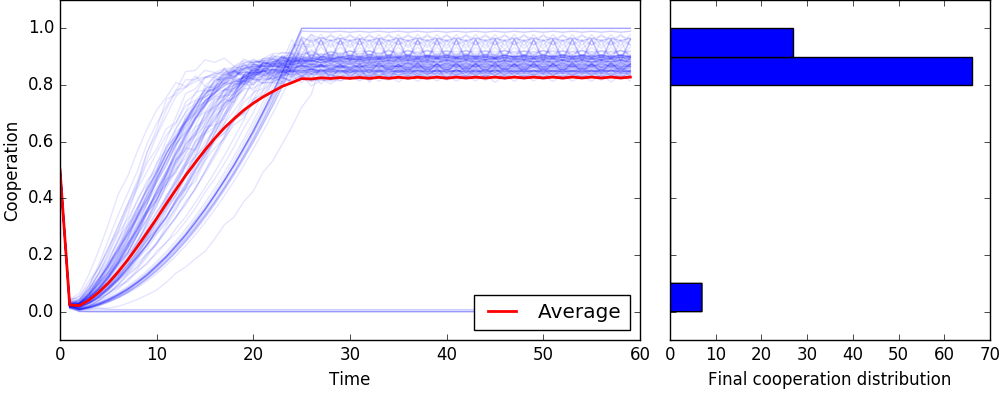
\includegraphics[width=0.7\textwidth]{./fig/n50.png}
	\caption{Cooperation levels of 100 runs along with their average
	on a 50x50 grid}
	\label{n50}
\end{figure}
Note that a stationary state does not necessarily mean that all simulations
have stopped moving. In fact, most of them reach a periodic equilibrium (as
can be seen with the sawteeth patterns appearing on figure \ref{n50}.\\

Most simulations reach a cooperation level between 80\% and 90\%. However, some
runs reach a total cooperation level while some dive very quickly to zero
cooperation.\\

Understanding the dynamics of this simulation starts by looking at figure
\ref{50viz}. When $t=5$, we clearly see clusters of cooperators (in magenta)
that expand until they meet other clusters (see when $t=10$). It makes sense
that these clusters expand because a defector right next to a single cluster
of cooperators will get a maximum payoff of $3T=30$ whereas a cooperator on 
the border of a cluster will get a payoff of $5R=35$; so the defector will
change his mind. This of course changes when two clusters meet : the defectors
stuck between two clusters will be able to take advantage of both clusters so
small trenches of defectors will remain and possibly oscillate as cooperators
want to take advantage of their cooperating neighbours.\\

A question remains: why do some runs delve to zero cooperation? This is
explained by the fact that the conditions for having a cluster are very harsh.
Indeed, in the first steps, most cooperators get wiped out unless they already
form a cluster large enough so that a core group of cooperators keeps
cooperating. A good example of this is the cluster that starts around the
coordinates (8,21).\\

\begin{figure}[H]
	\centering
	\subfloat[][$t=0$]{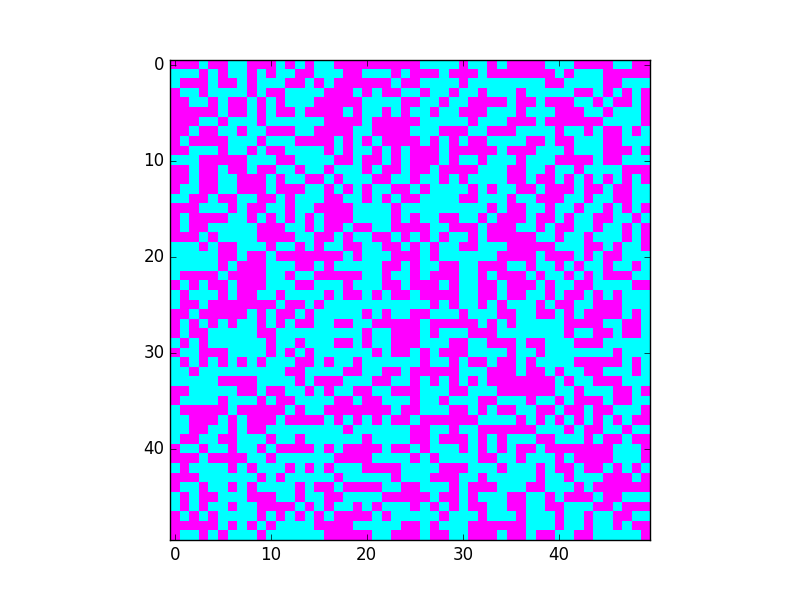
\includegraphics[width=.3\textwidth]{./fig/s0.png}}
	\subfloat[][$t=1$]{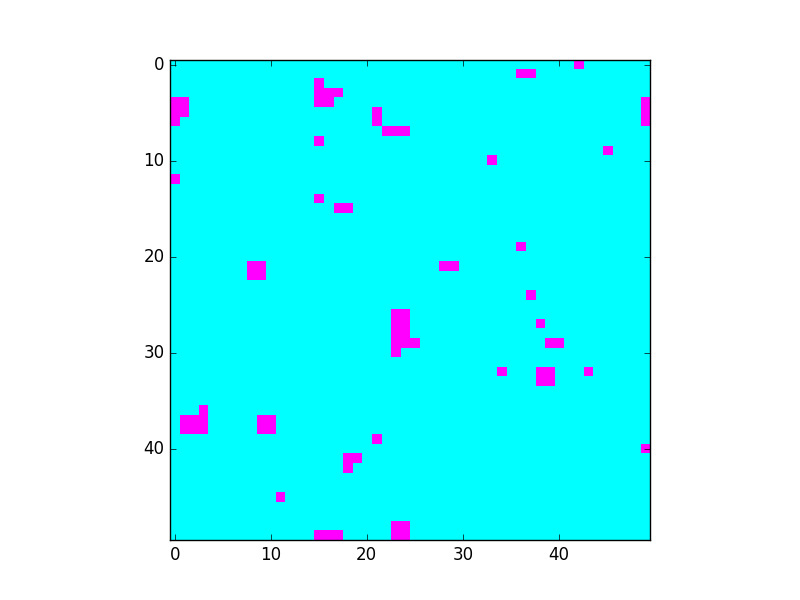
\includegraphics[width=.3\textwidth]{./fig/s1.png}}
	\subfloat[][$t=5$]{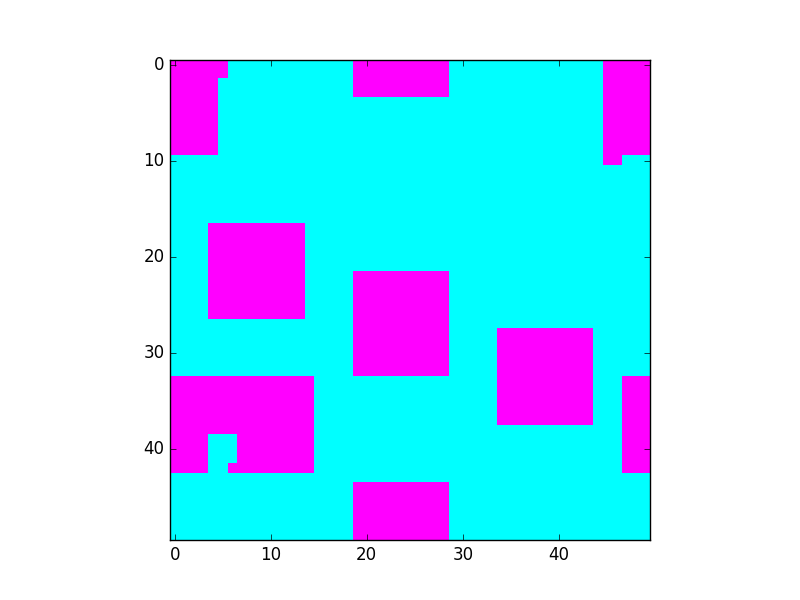
\includegraphics[width=.3\textwidth]{./fig/s5.png}}
	\\
	\subfloat[][$t=10$]{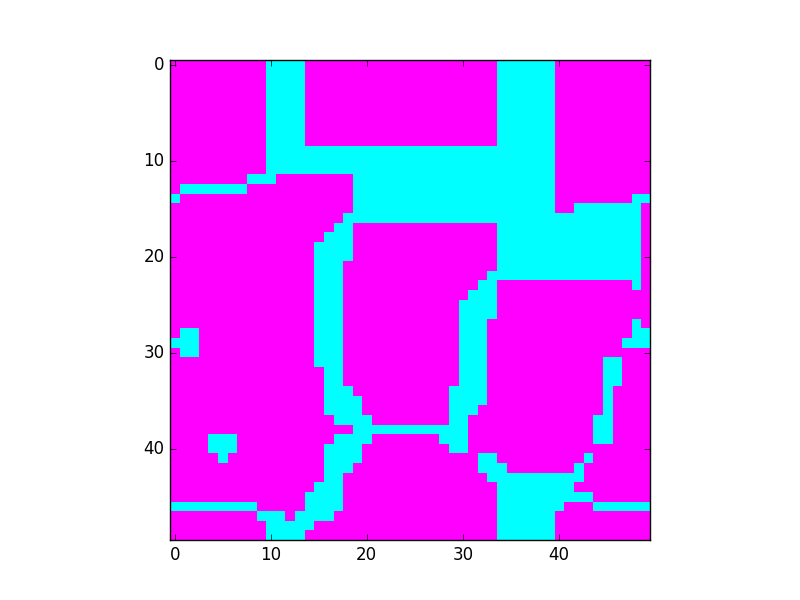
\includegraphics[width=.3\textwidth]{./fig/s10.png}}
	\subfloat[][$t=20$]{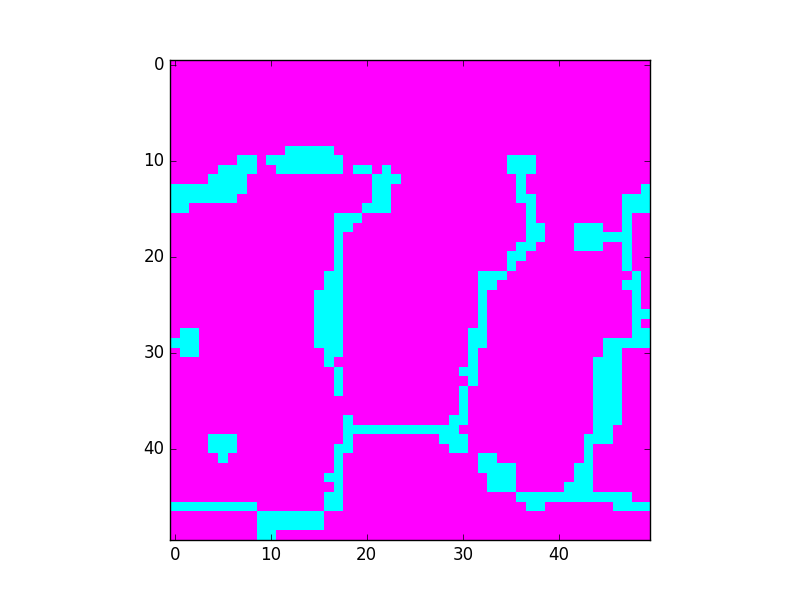
\includegraphics[width=.3\textwidth]{./fig/s20.png}}
	\subfloat[][$t=50$]{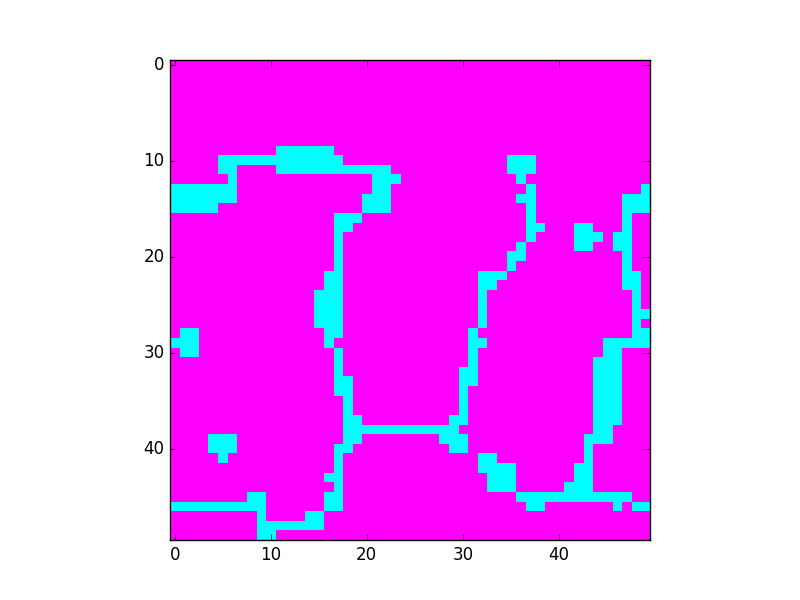
\includegraphics[width=.3\textwidth]{./fig/s50.png}}
	\caption{Evolution of one run on a 50x50 grid with defectors in cyan
	and cooperators in magenta}
	\label{50viz}
\end{figure}

This is exactly why, for a grid of size 4x4, the cooperation average is 
very close to zero : as clusters are fairly unlikely at the start and since
we don't have as many positions to start with (16 compared to 2500), the
probability of having a cluster is only 16/2500 times the one of a 50x50
grid. In fact, most runs of a 4x4 grid will end up falling to only defectors
after the second iteration (see figures \ref{4viz} and \ref{pr_m_convs}a).\\

\begin{figure}[H]
	\centering
	\subfloat[][$t=0$]{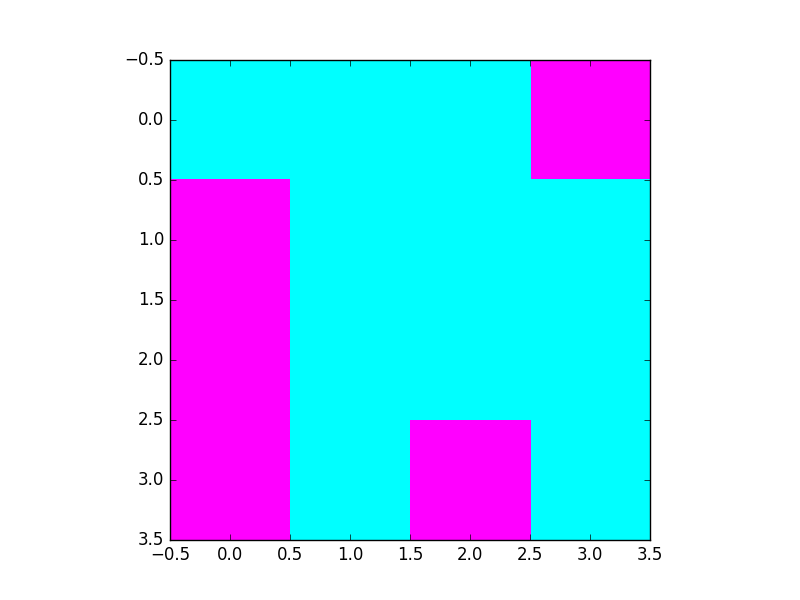
\includegraphics[width=.3\textwidth]{./fig/s4_0.png}}
	\subfloat[][$t=1$]{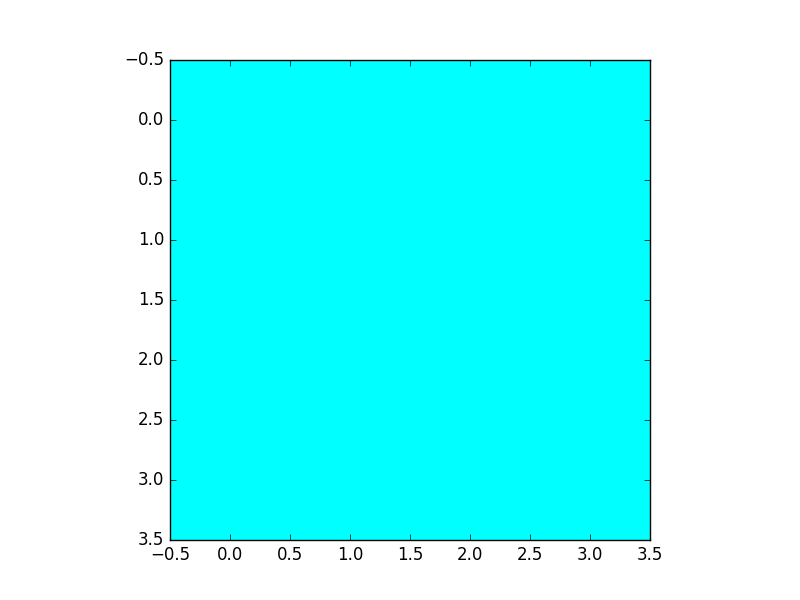
\includegraphics[width=.3\textwidth]{./fig/s4_1.png}}
	\caption{Evolution of one run on a 4x4 grid}
	\label{4viz}
\end{figure}

One thing worth noting, however, is that when the conditions are sufficient to
generate a cluster, the level of cooperation reached will always be around
80\%; only the proportion of simulations that reach it (instead of falling to
zero) changes. It is very clearly shown on figure \ref{pr_m_convs}).\\

We could say that the two modes of the bimodal distribution describing the 
final cooperation level never change; only the number of simulations belonging
to each mode changes, and the larger the grid is, the larger the number of 
simulations finishing with a high cooperation level will be.\\

Another observation, although trivial, would be to note that for smaller grids
that reach cooperation, the convergence is quicker as the clusters do not have
to grow for as much time as the larger grids before meeting either other
clusters or themselves because of the periodic boundary conditions.

\begin{figure}[H]
	\centering
	\subfloat[][4x4]{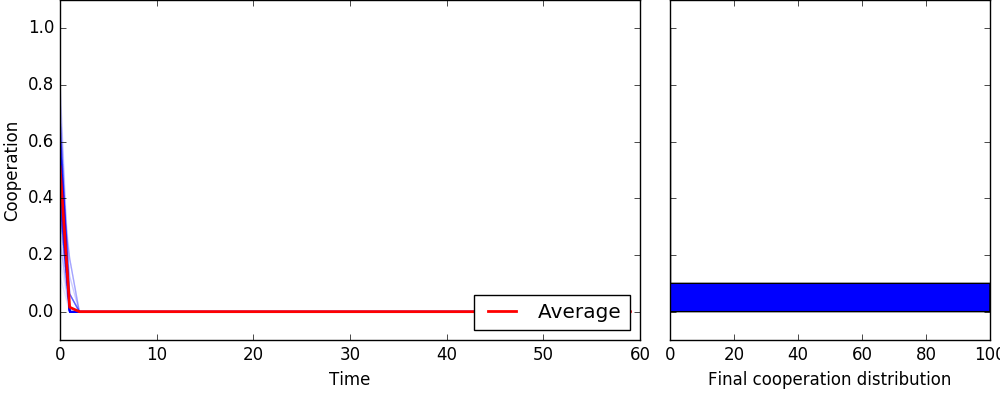
\includegraphics[width=.5\textwidth]{./fig/n4.png}}
	\subfloat[][8x8]{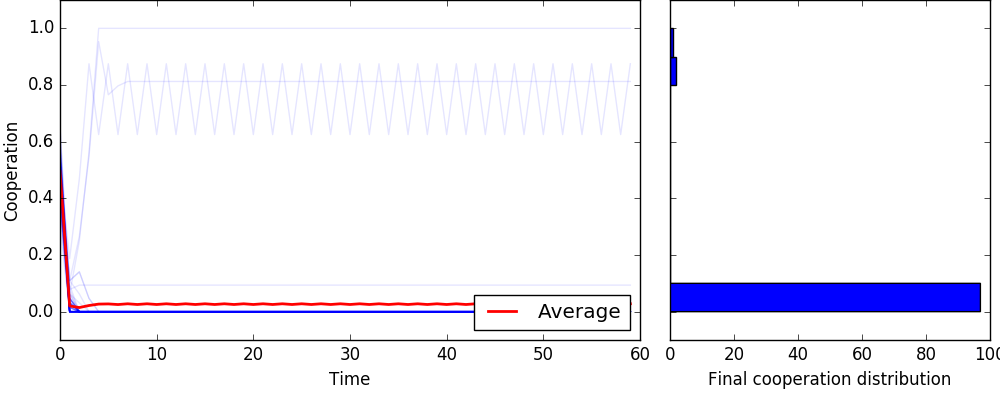
\includegraphics[width=.5\textwidth]{./fig/n8.png}}
	\\
	\subfloat[][12x12]{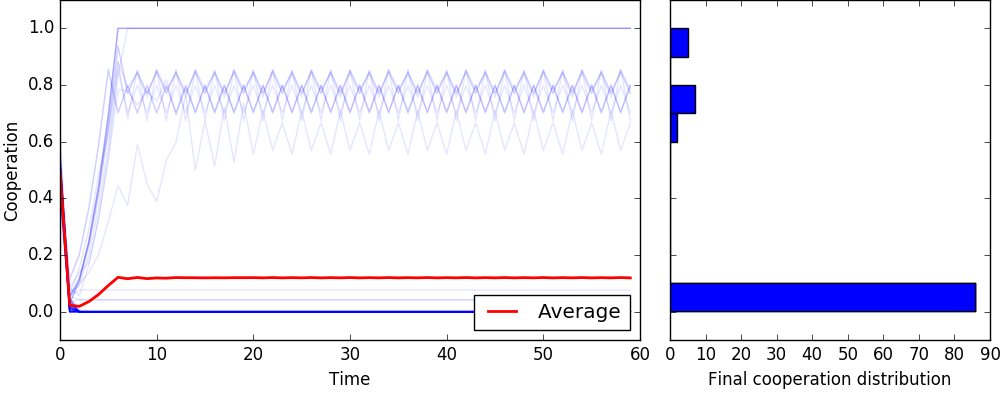
\includegraphics[width=.5\textwidth]{./fig/n12.png}}
	\subfloat[][20x20]{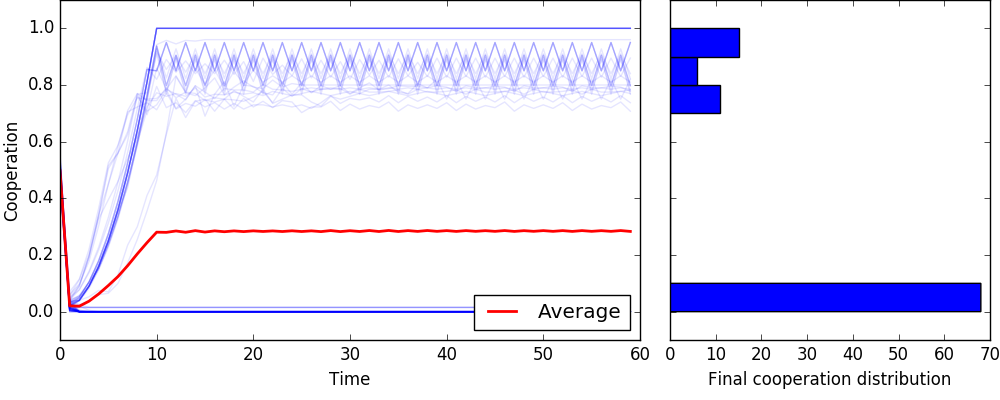
\includegraphics[width=.5\textwidth]{./fig/n20.png}}
	\caption{Variation of the convergence of runs with the grid size}
	\label{pr_m_convs}
\end{figure}

\subsection{Von Neumann neighbourhood}
Figure \ref{vn50} shows the convergence levels with the Von Neumann
neighbourhood. There are some striking differences with the Moore neighbourhood.
First, the average convergence level is much lower, at around 40\%, and second,
the runs do not seem to stabilise as much as with the Moore neighbourhood; 
their period seems to be much longer. Also, no run makes it to 100\% or 0\%
cooperation. They all stay very close to 40\% cooperation. 

\begin{figure}[H]
	\centering
	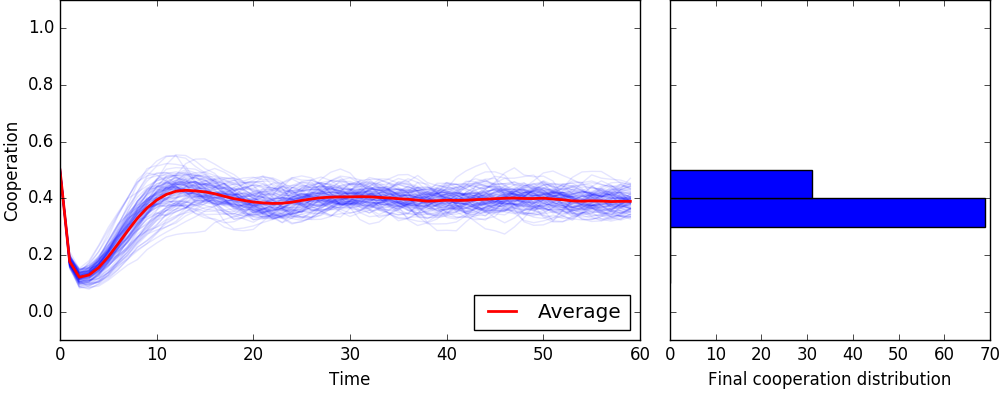
\includegraphics[width=0.7\textwidth]{./fig/vn_50.png}
	\caption{Cooperation levels of 100 runs along with their average
	on a 50x50 grid with the Von Neumann neighbourhood}
	\label{vn50}
\end{figure}

Let us try to understand why this is happening by looking at an example run
on figure \ref{vnviz}.

\begin{figure}[H]
	\centering
	\subfloat[][$t=0$]{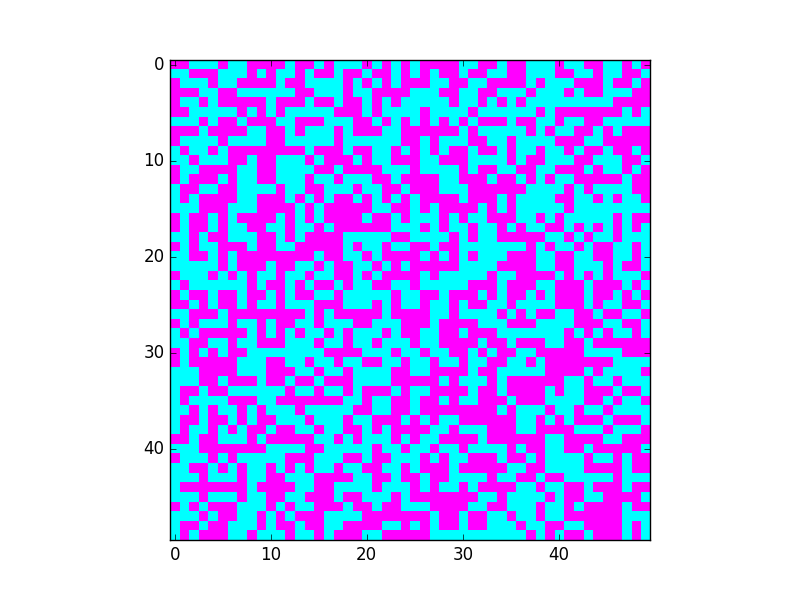
\includegraphics[width=.3\textwidth]{./fig/vn_s0.png}}
	\subfloat[][$t=1$]{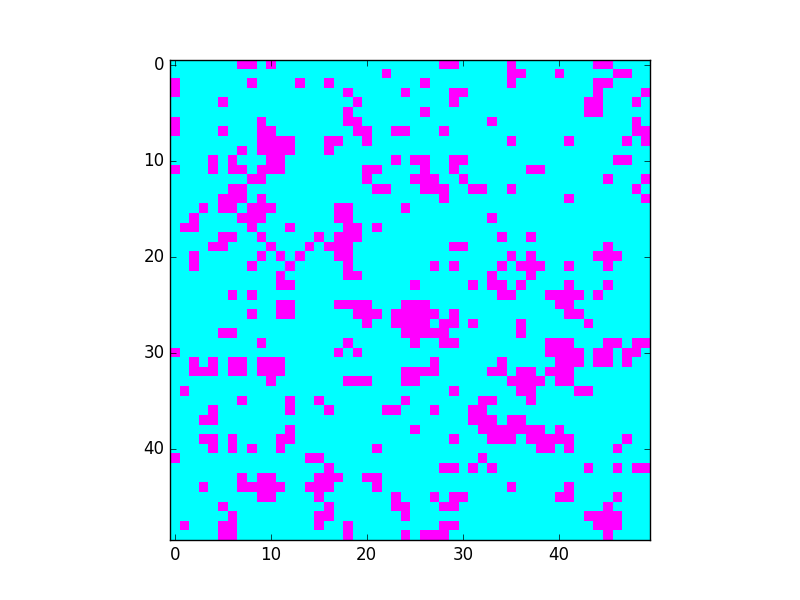
\includegraphics[width=.3\textwidth]{./fig/vn_s1.png}}
	\subfloat[][$t=5$]{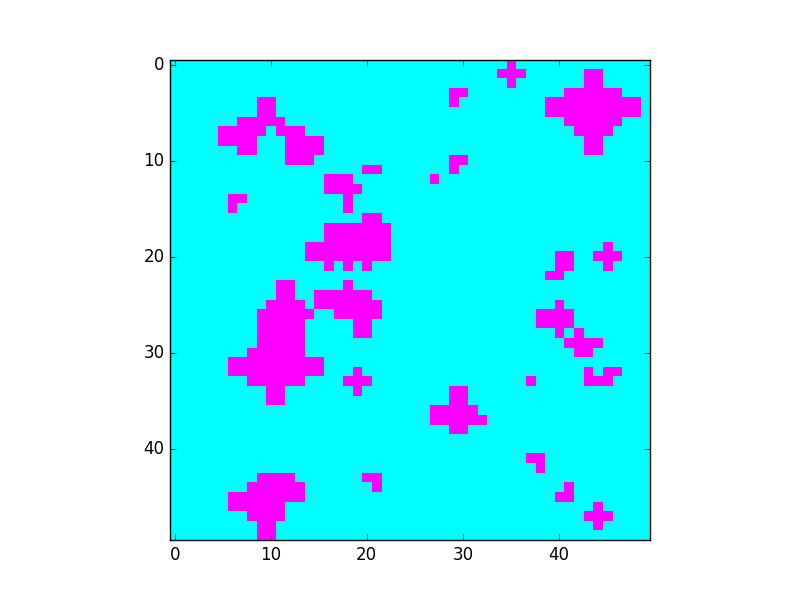
\includegraphics[width=.3\textwidth]{./fig/vn_s5.png}}
	\\
	\subfloat[][$t=10$]{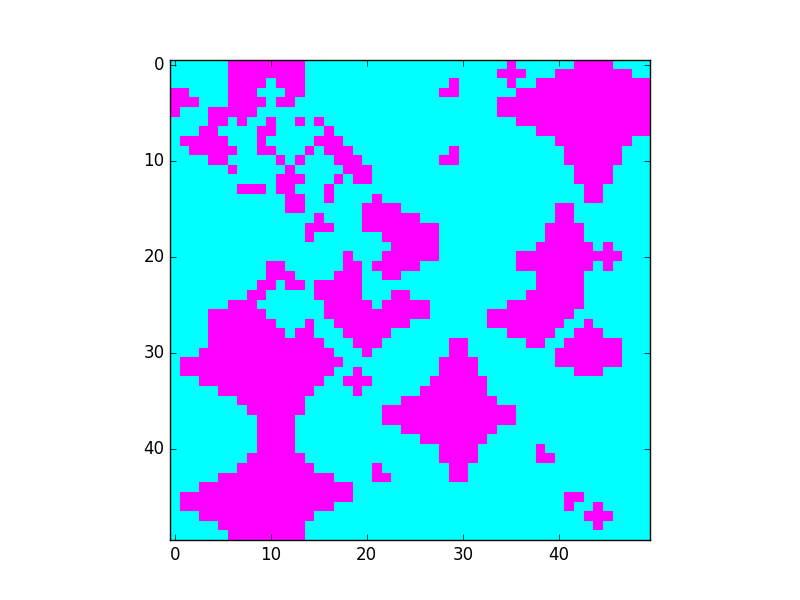
\includegraphics[width=.3\textwidth]{./fig/vn_s10.png}}
	\subfloat[][$t=20$]{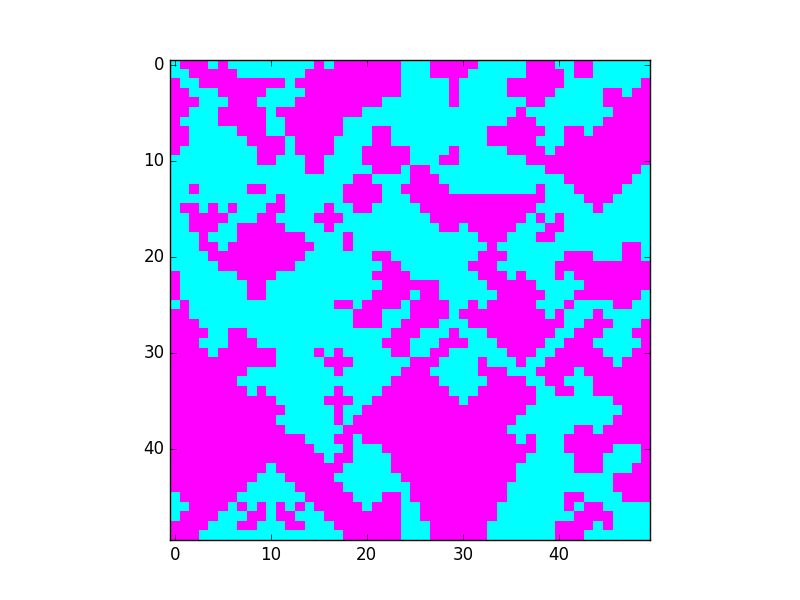
\includegraphics[width=.3\textwidth]{./fig/vn_s20.png}}
	\subfloat[][$t=50$]{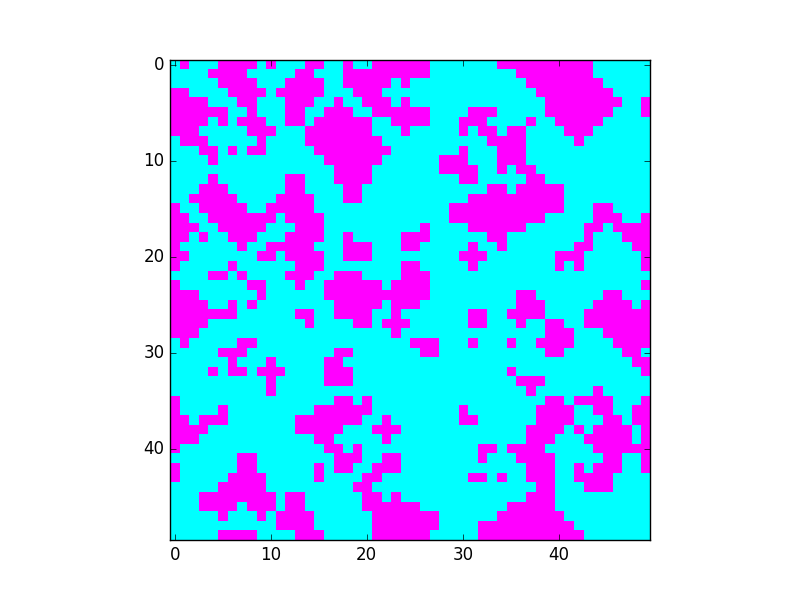
\includegraphics[width=.3\textwidth]{./fig/vn_s50.png}}
	\caption{Evolution of one run on a 50x50 grid with the Von Neumann
	Neighbourhood}
	\label{vnviz}
\end{figure}

A first noticeable difference is that the boundaries between cooperators and
defectors are now more diagonal rather than horizontal or vertical. In the 
case of the Von Neumann neighbourhood, once the original clusters have 
expanded, it becomes more interesting for the cooperators on the border of
a cluster near another one to become a defector, so the boundaries between
clusters will start growing again while clusters of cooperators will continue
expanding into defector-only regions, creating an endlessly moving pattern.


\section{The snowdrift game}
The snowdrift game is the following :
\begin{table}[H]
\centering
\begin{tabular}{c|cc|cc}
	& \multicolumn{2}{c|}{\textbf{C}} & \multicolumn{2}{c}{\textbf{D}}\\
	\hline
	\textbf{C} && 7 && 10\\
	& 7 && 3 &\\
	\hline
	\textbf{D} && 3 && 0\\
	& 10 && 0 &\\
\end{tabular}
\end{table}
Let us try to understand why we set up the probability $p_{ij}$ with the
following formula :

$$ p_{ij} = \frac{
	1 + \frac{W_j-W_i}{N(\text{max}(P,R,T,S)-\text{min}(P,R,T,S))}
	}
	{2}$$

The inner denominator $N(\text{max}(P,R,T,S)-\text{min}(P,R,T,S))$
normalises $W_j-W_i$ to contain it between -1 and 1. We then clearly 
understand that $p_{ij}$ will be contained between 0 and 1. It makes sense
to use this formula because the only variables are $W_j$ and $W_i$ : the higher
the difference is between the two, the higher the probability of picking the 
best payoff will be. If both payoffs are equal, $p_{ij} = \frac{1}{2}$ so 
we will choose either one at random.

\subsection{Moore neighbourhood comparison}
There are several key trends to notice on figure \ref{conv_sd}:
\begin{enumerate}
	\item The bimodality of the final cooperation distribution evolves; 
		early on, there is only one mode but as simulations manage to
		reach either full or zero cooperation, two modes emerge
	\item In the prisoners dilemma, the average for the runs reaching a
		non-zero cooperation level was around 85\% percent; in this
		case, it is harder to estimate. as it looks like the cooperation
		converges at 40\% for large grids, but we could argue that 
		this level could change much later as the simulations reach
		100\% or 0\% cooperation just like in the case of the 4x4 grid
	\item \textbf{Perhaps the most interesting one}, the standard 
		deviation of the final cooperation distribution seems to
		decrease as the size of the grid grows.
\end{enumerate}

\begin{figure}[H]
	\centering
	\subfloat[][4x4]{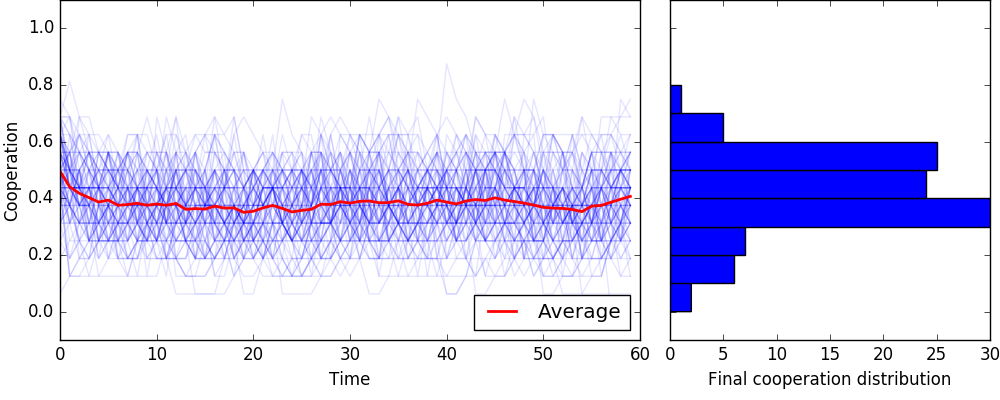
\includegraphics[width=.5\textwidth]{./fig/sd_n4.png}}
	\subfloat[][8x8]{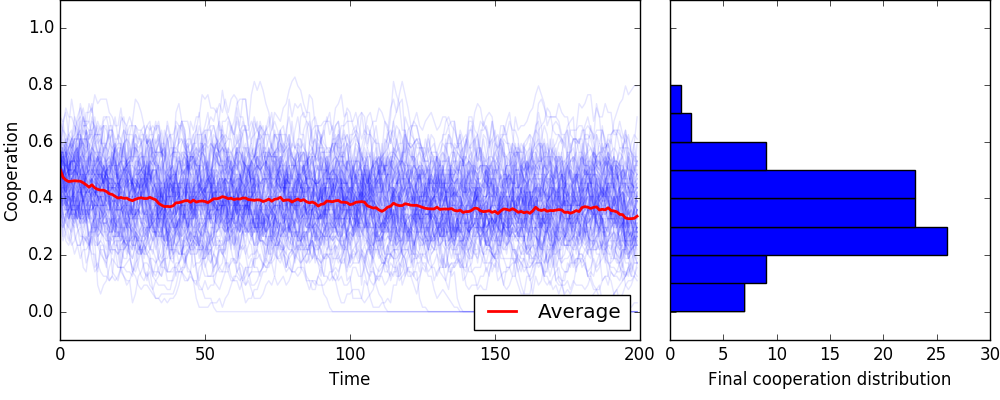
\includegraphics[width=.5\textwidth]{./fig/sd_n8.png}}\\
	\subfloat[][12x12]{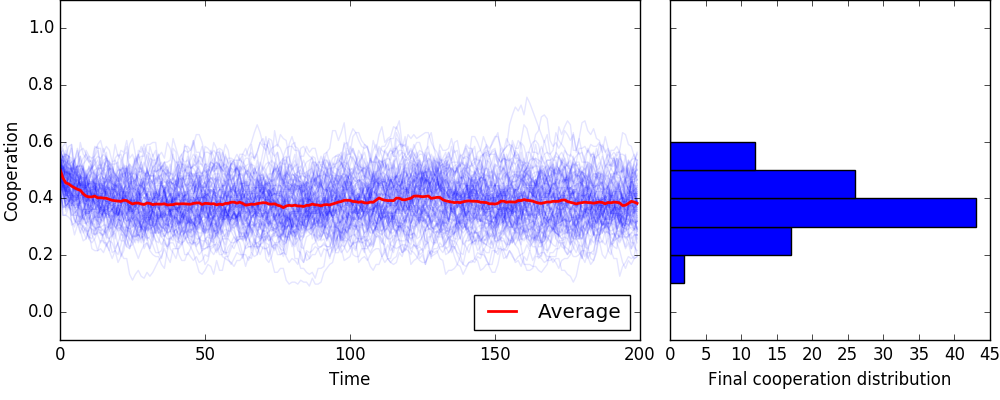
\includegraphics[width=.5\textwidth]{./fig/sd_n12.png}}
	\subfloat[][20x20]{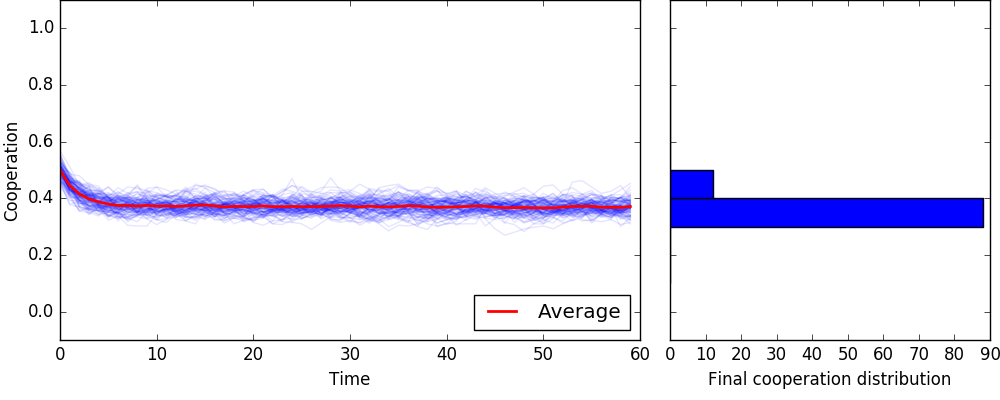
\includegraphics[width=.5\textwidth]{./fig/sd_n20.png}}\\
	\subfloat[][50x50]{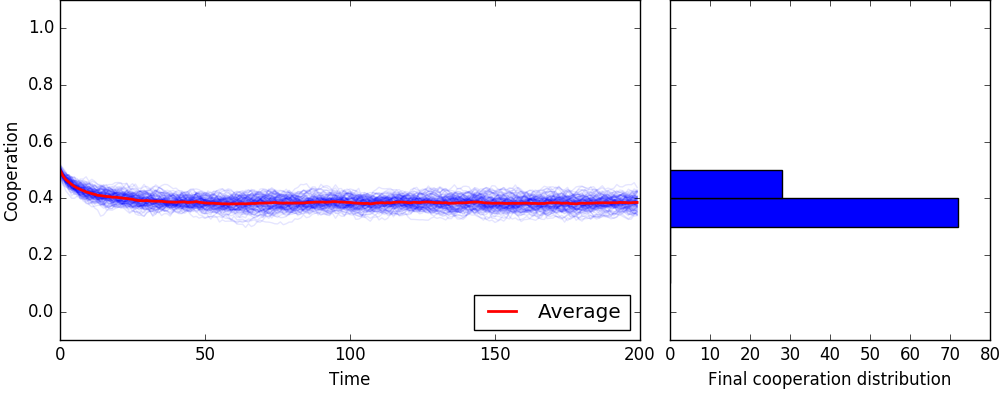
\includegraphics[width=.5\textwidth]{./fig/sd_n50.png}}
	\caption{Convergence of 100 runs for various grid sizes with the Moore
	neighbourhood}
	\label{conv_sd}
\end{figure}

Intuitively, it makes sense that the equilibrium state is around 40\%. If a 
cooperator is surrounded by defectors, it will still get a payoff of 24 with the
Moore neighbourhood while all the defectors will get 10, so the defectors will
have a tendency to start cooperating. However, if a defector is surrounded by
cooperators, it will get the highest payoff and the cooperators will have a 
tendency to start defecting. The reason why the equilibrium is lower than 50\%
is that defecting gives a higher payoff than cooperating. \\

The reason why the standard deviation seems to decrease as we increase the grid 
size can be explained by the law of large numbers. Just like when we flip a
coin many times, the probability of having only heads is very low, 
the probability of a quarter of the cells choosing to defect at the same time
is not so low for the 4x4 grid but is quite low for the 50x50 grid. \\

However, we could expect that after a very long time, all the runs will end up
taking a path that will take them to 100\% or 0\% cooperation. As the grid
grows larger, this path becomes more and more unlikely of course, and this is
why we see the runs converging to 100\% and 0\% on the 4x4 grid, and we start
seeing runs converging to 0\% on the 8x8 grid. This is only a hypothesis 
though.\\

Let us now look at a run.

\begin{figure}[H]
	\centering
	\subfloat[][$t=0$]{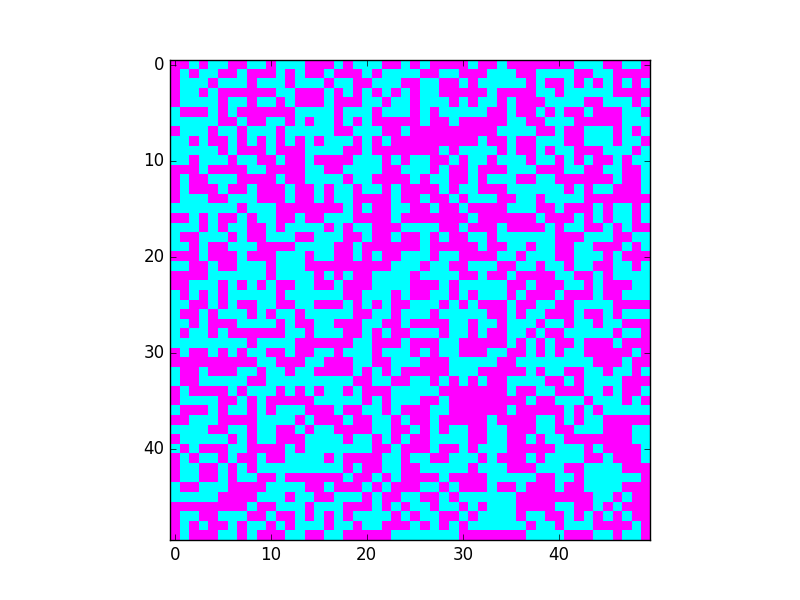
\includegraphics[width=.3\textwidth]{./fig/sd_s0.png}}
	\subfloat[][$t=1$]{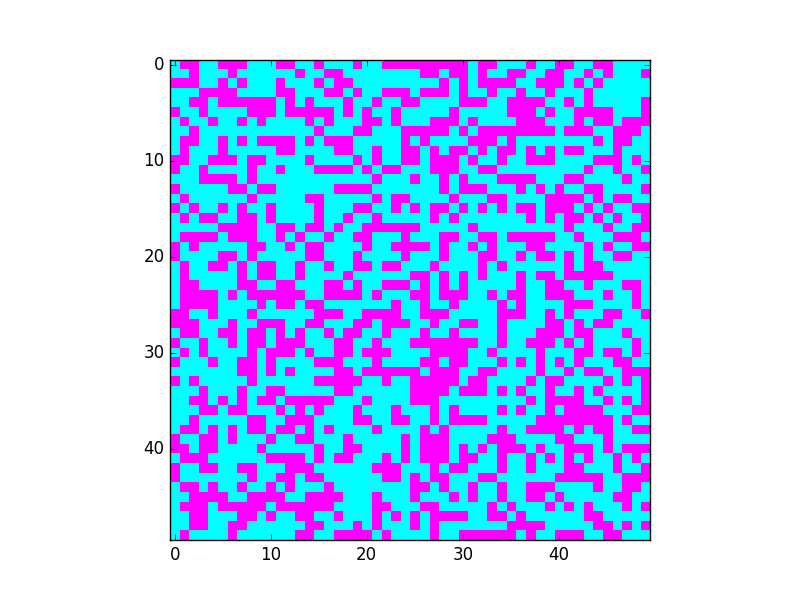
\includegraphics[width=.3\textwidth]{./fig/sd_s1.png}}
	\subfloat[][$t=5$]{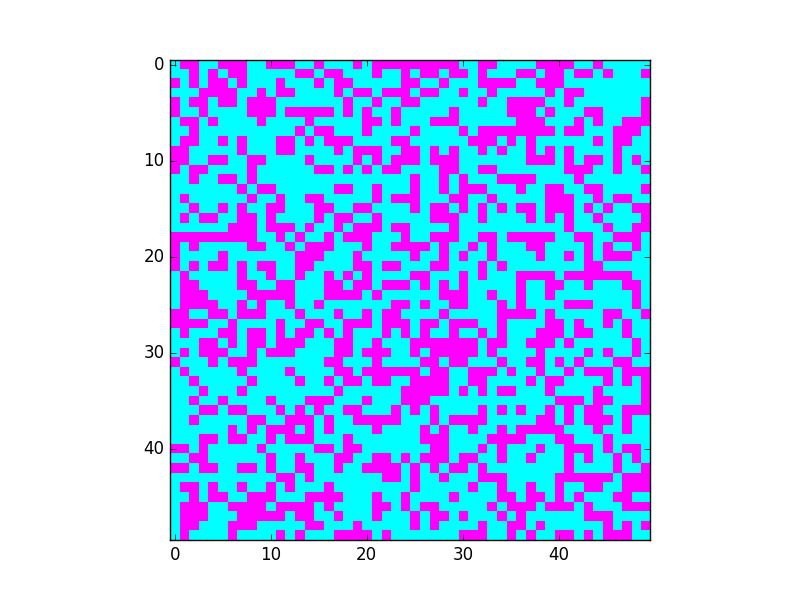
\includegraphics[width=.3\textwidth]{./fig/sd_s2.png}}
	\\
	\subfloat[][$t=10$]{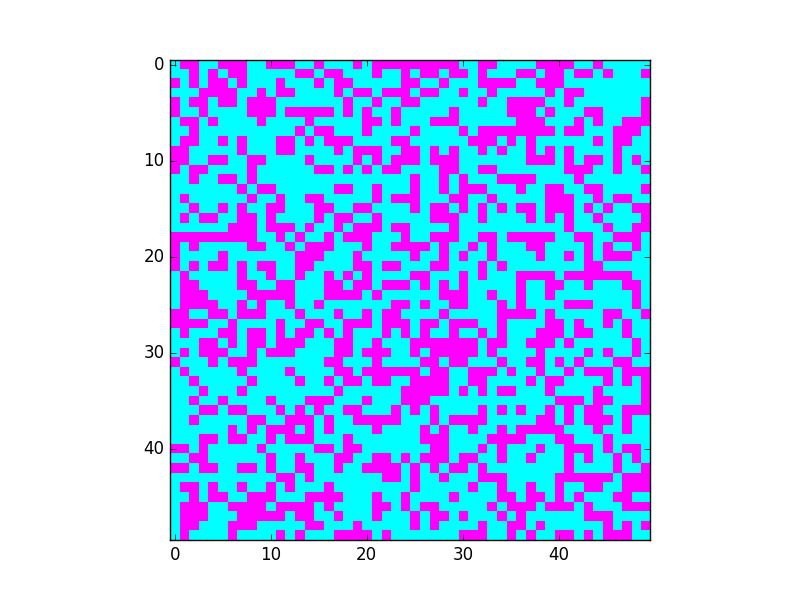
\includegraphics[width=.3\textwidth]{./fig/sd_s3.png}}
	\subfloat[][$t=20$]{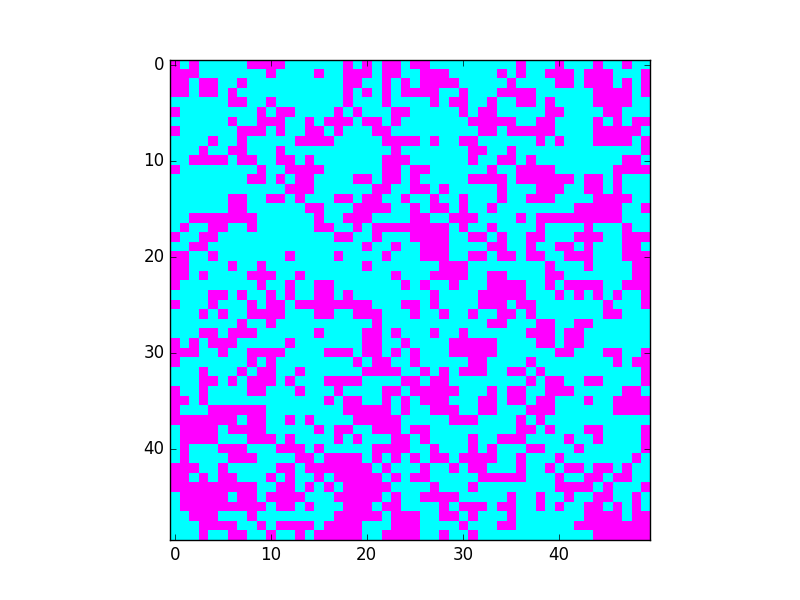
\includegraphics[width=.3\textwidth]{./fig/sd_s4.png}}
	\subfloat[][$t=50$]{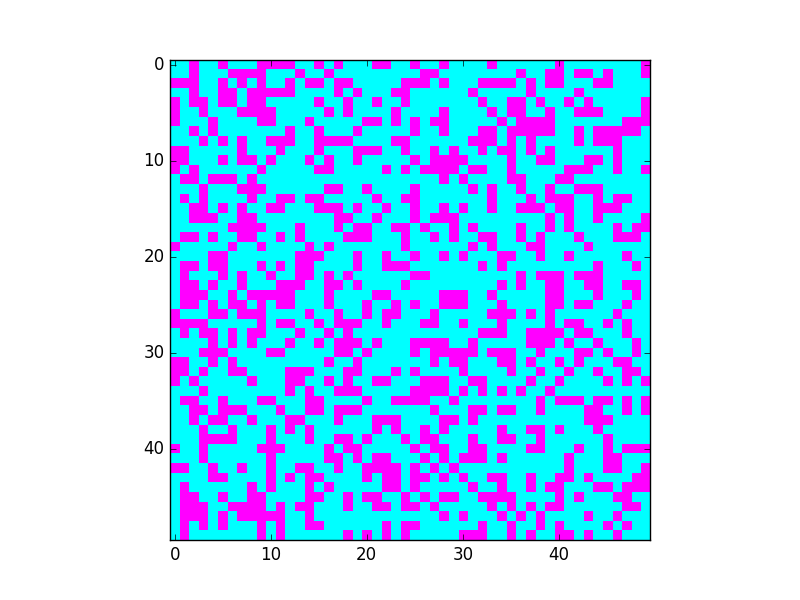
\includegraphics[width=.3\textwidth]{./fig/sd_s5.png}}
	\caption{Evolution of one run on a 50x50 grid with the snowdrift game
	and the Moore neighbourhood}
	\label{sdrun}
\end{figure}

We can indeed see that the grid doesn't change too much from one iteration to
the next. This is partly due to the fact that in the case where a neighbouring
cell has a higher payoff than us (which is not necessarily the case), we might
not pick it as our comparison cell, and if we do pick it, we won't copy the
neighbouring cell's behaviour with certainty.

\subsection{Von Neumann neighbourhood}
Figure \ref{sd_vn50} shows that the Von Neumann neighbourhood impacts not
only the speed at which the simulations converge to a stationary state, but
also the cooperation level average at convergence; which is at 20\% instead
of 40\%. 
\begin{figure}[H]
	\centering
	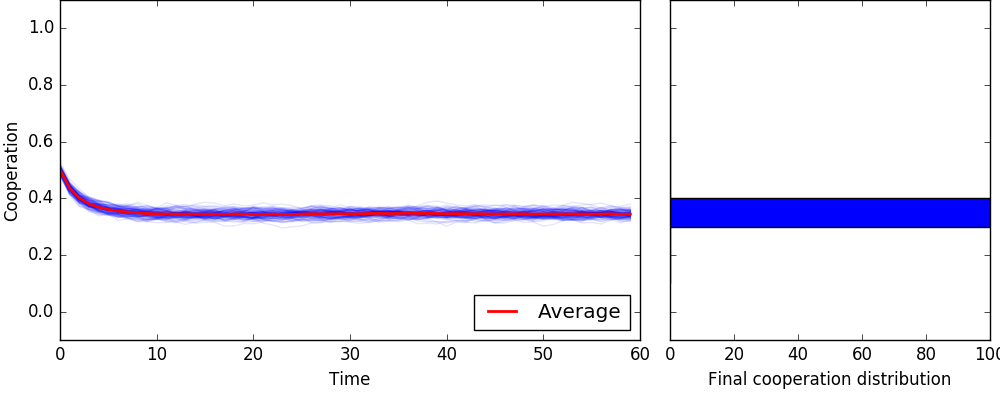
\includegraphics[width=0.7\textwidth]{./fig/sd_vn_50.png}
	\caption{Cooperation levels of 100 runs along with their average
	on a 50x50 grid for the snowdrift game with a Von Neumann neighbourhood}
	\label{sd_vn50}
\end{figure}

\section{Sidenote}
As a bonus, here is a way to reach 50\% cooperation, and also, a very 
convoluted and complicated way of scaling and rotating a pink square using
the prisoners dilemma game with the Von Neumann neighbourhood, all the while
going through an arguably amazing animation : 

\begin{figure}[H]
	\centering
	\subfloat[][]{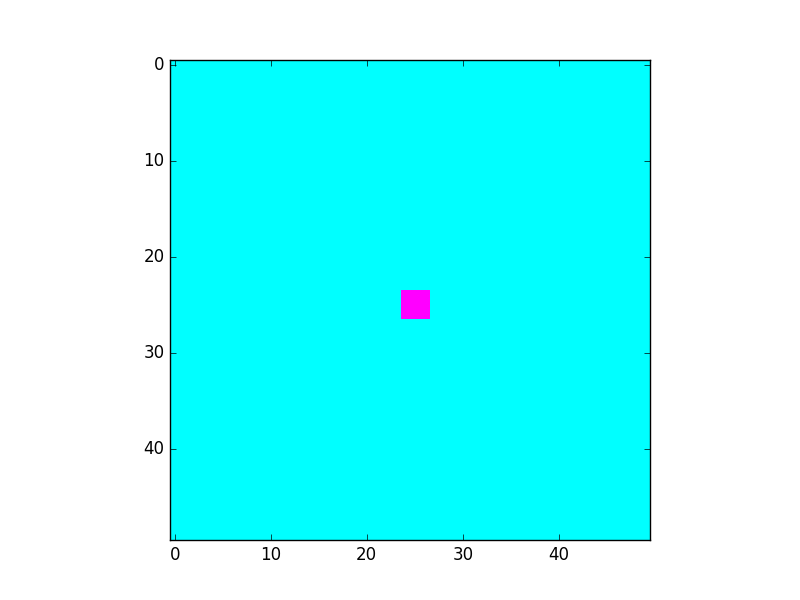
\includegraphics[width=.3\textwidth]{./fig/fun_0.png}}
	\subfloat[][]{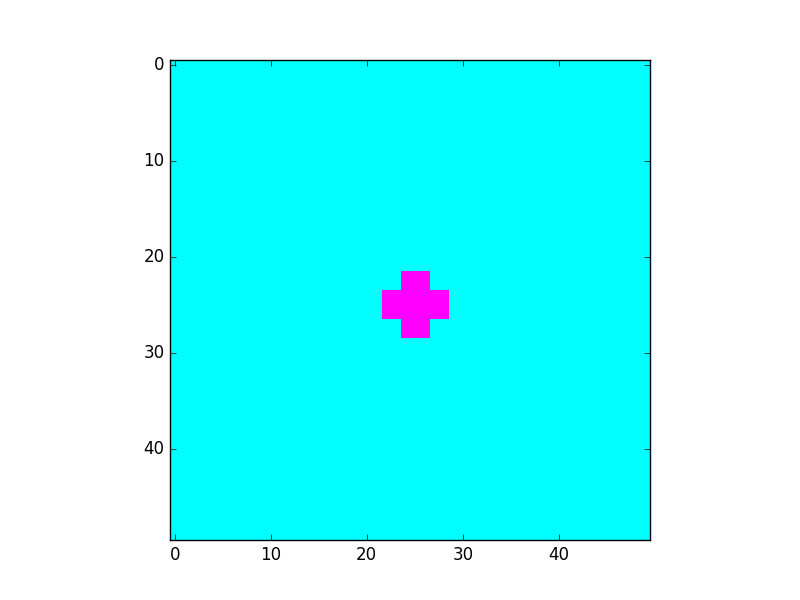
\includegraphics[width=.3\textwidth]{./fig/fun1.png}}
	\subfloat[][]{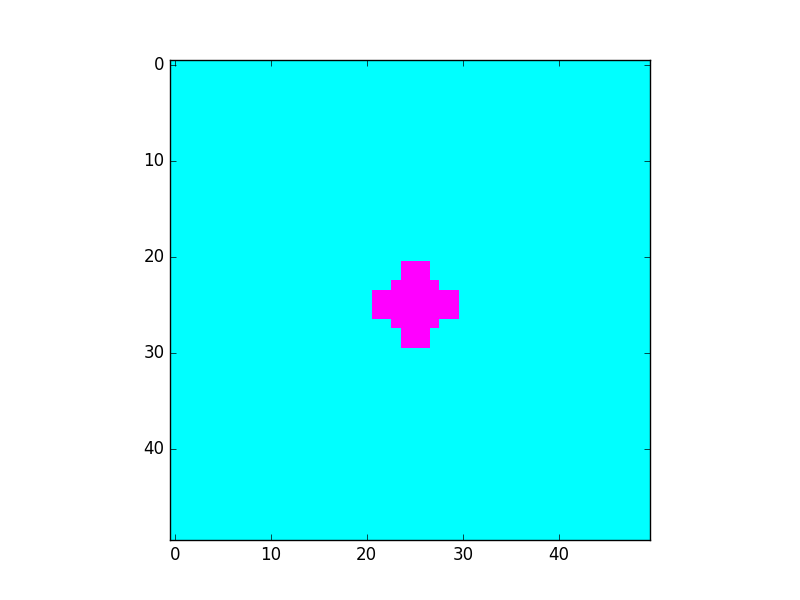
\includegraphics[width=.3\textwidth]{./fig/fun3.png}}
	\\
	\subfloat[][]{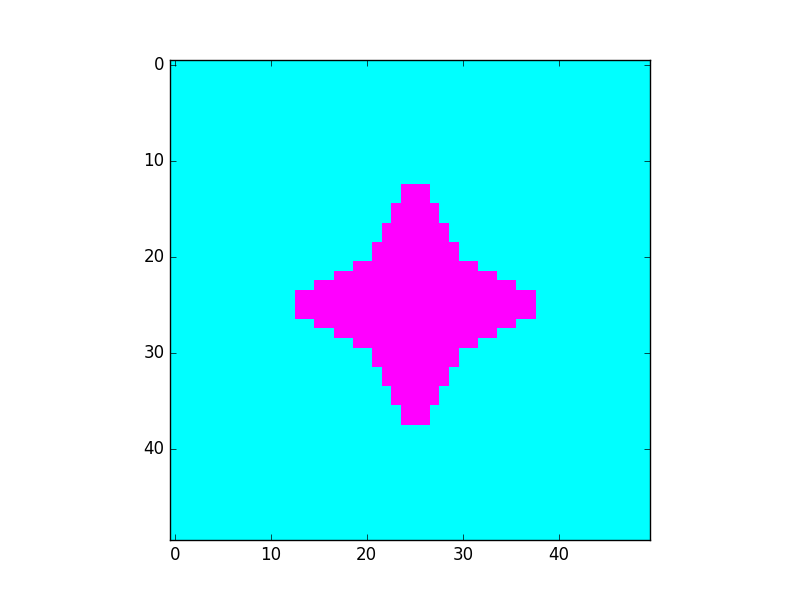
\includegraphics[width=.3\textwidth]{./fig/fun4.png}}
	\subfloat[][]{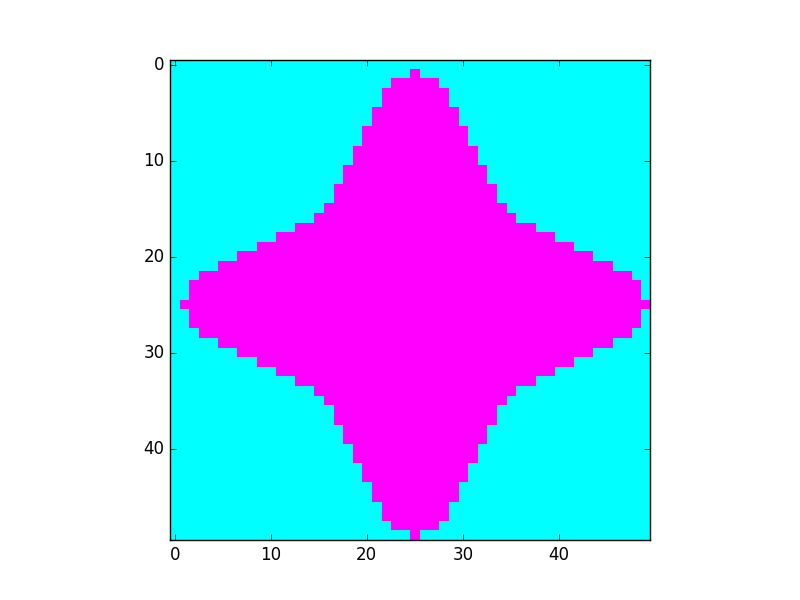
\includegraphics[width=.3\textwidth]{./fig/fun6.png}}
	\subfloat[][]{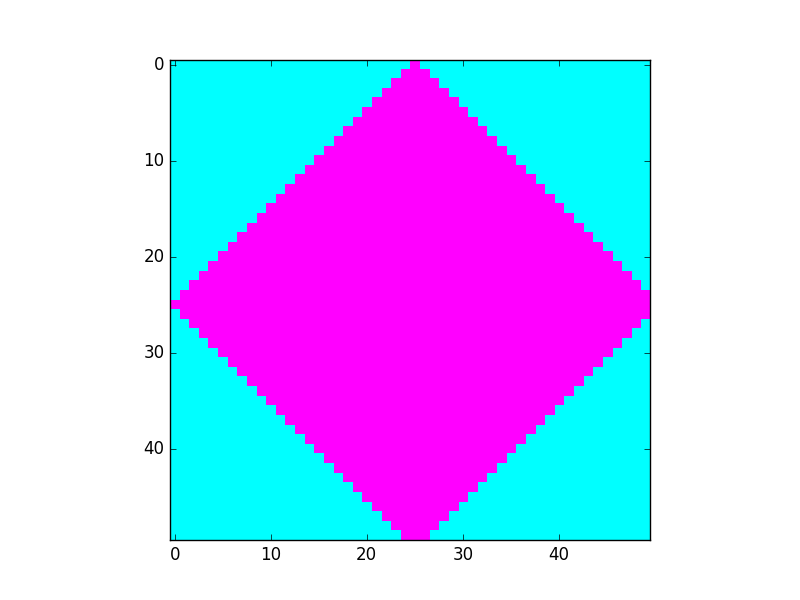
\includegraphics[width=.3\textwidth]{./fig/fun8.png}}
	\caption{A truly awe-inspiring animation}
	\label{sdrun}
\end{figure}
\end{document}
